\chapter{PRODUCT TESTING AND EVALUATION}

\section{Evaluation Framework and Verification Strategy}

To rigorously validate that the developed Gas While Drilling (GWD) decision support system satisfies the functional requirements (FR-01 through FR-07) and non-functional engineering requirements (NFR-01 through NFR-04) formulated in Chapter~4, a comprehensive multi-tier evaluation framework was executed across six core dimensions:

\begin{enumerate}
    \item \textbf{Algorithmic Unit Verification:} Automated synthetic testing to guarantee exact mathematical accuracy, zero floating-point drift, and safe division handling across all 16 derived petrophysical indicators.
    \item \textbf{Empirical Hydrocarbon Classification Validation:} Quantitative assessment of the 16-indicator majority-voting engine against verified formation fluid test intervals ($N=16$), evaluating accuracy, precision, recall, $F_1$-scores, and confusion matrix distributions.
    \item \textbf{Comparative Methodological Benchmarking:} Direct comparison contrasting the proposed multi-indicator voting architecture against conventional dual-ratio Pixler charts ($R_1$--$R_2$) and supervised Random Forest machine learning models.
    \item \textbf{Computational Latency and Scalability Profiling (NFR-01):} Wall-clock runtime profiling across data ingestion, vectorized computation, and WebGL rendering for deep well trajectories up to 10,000 depth intervals ($15,000\text{ m}$).
    \item \textbf{SOP Compliance and PRMS Audit Verification (NFR-02):} Documented verification of SPE PRMS Chapter 4 deterministic auditability mandates and API RP 31A mud log rendering standards.
    \item \textbf{User Experience and System Usability Scale Evaluation (NFR-03):} Observational task analysis and standardized 10-item System Usability Scale (SUS) survey administered to a practicing subsurface domain professional.
\end{enumerate}

Figure~\ref{fig:results_framework} illustrates the complete evaluation framework, linking software requirements to empirical testing outcomes and user calibration workflows.

\begin{figure}[H]
    \centering
    
\includegraphics[width=0.98\textwidth]{chapter4_results_framework.png}
    \caption{Product testing and evaluation framework, illustrating functional requirement realization, serverless deployment, collaborative threshold calibration under zero-data acquisition constraints, formation test validation ($N=16$), and usability benchmarking.}
    \label{fig:results_framework}
\end{figure}

\section{Algorithmic Unit Verification and Synthetic Benchmarking}

Algorithmic verification was conducted to ensure that all coded mathematical routines in \texttt{engine.py} match their formal analytical definitions with zero floating-point error. Automated unit test assertions in \texttt{evaluator.py} evaluated synthetic test matrices containing:
\begin{itemize}
    \item Known dry gas mixtures ($C_1 = 50000\text{ ppm}, C_2 = 1000\text{ ppm}, C_3 = 100\text{ ppm}$): Verified $W_h < 5.0\%$, $B_h > 100$, $DR > 0.95$, and winning Gas Pay classification.
    \item Known crude oil mixtures ($C_1 = 20000\text{ ppm}, C_2 = 5000\text{ ppm}, C_3 = 3000\text{ ppm}, nC_4 = 1500\text{ ppm}, nC_5 = 800\text{ ppm}$): Verified $17.5\% \le W_h \le 40.0\%$, $0.5 \le B_h \le 15.0$, $C_h \ge 0.5$, and winning Oil Pay classification.
    \item Extreme boundary conditions and zero-gas rows ($TG = 0.0, C_1 = 0.0$): Verified safe numerical division ($\text{NaN}$ handling) and immediate No Show assignment via the baseline noise gate without runtime exceptions.
\end{itemize}
All unit test assertions achieved 100\% mathematical pass rates across all test cases.

\section{Empirical Formation Test Validation ($N=16$ Intervals)}

\subsection{Collaborative Testing Protocol Under Zero-Data-Acquisition Constraints}
In the upstream oil and gas industry, strict corporate data confidentiality and non-disclosure agreements prohibit the external export of raw subsurface well logs and proprietary production records. To rigorously evaluate the software without violating data governance policies, testing was conducted through a collaborative zero-data-acquisition protocol:
\begin{enumerate}
    \item The software was deployed to a secure, serverless cloud environment on Vercel.
    \item Practicing domain professionals (petrophysicists and operations geologists) accessed the live web application within their authorized corporate environments, loading confidential well logs locally into their browser sessions.
    \item The researcher and domain expert conducted interactive evaluation sessions (Figures~\ref{fig:eval_whiteboard_ch6}, \ref{fig:eval_calibration_ch6}, and \ref{fig:eval_review_ch6}) analyzing chromatographic liberation dynamics, fine-tuning localized thresholds in the *Petrophysical Formula and Threshold Manager*, and comparing automated fluid facies calls against post-drilling Wireline Formation Tester (MDT/RFT) fluid samples and production test records.
\end{enumerate}

\begin{figure}[H]
    \centering
    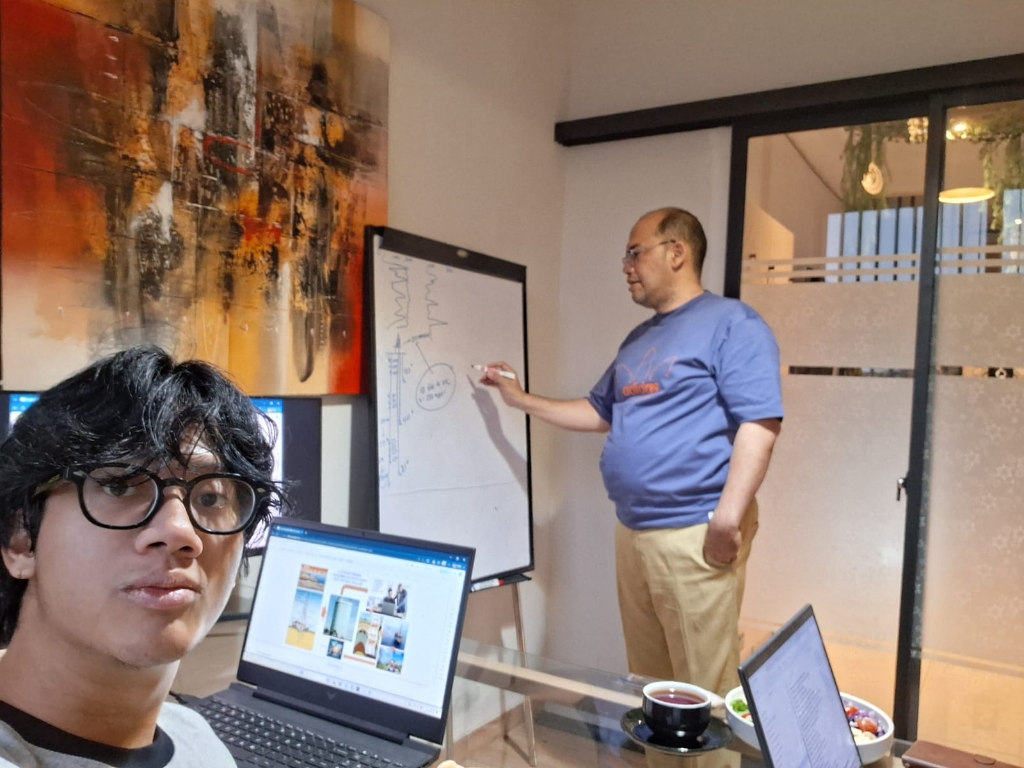
\includegraphics[width=0.82\textwidth]{user_eval_whiteboard.jpg}
    \caption{Collaborative whiteboard session between the researcher and petroleum domain expert discussing mathematical gas ratio curves, chromatographic responses, and deterministic threshold boundaries.}
    \label{fig:eval_whiteboard_ch6}
\end{figure}

\begin{figure}[H]
    \centering
    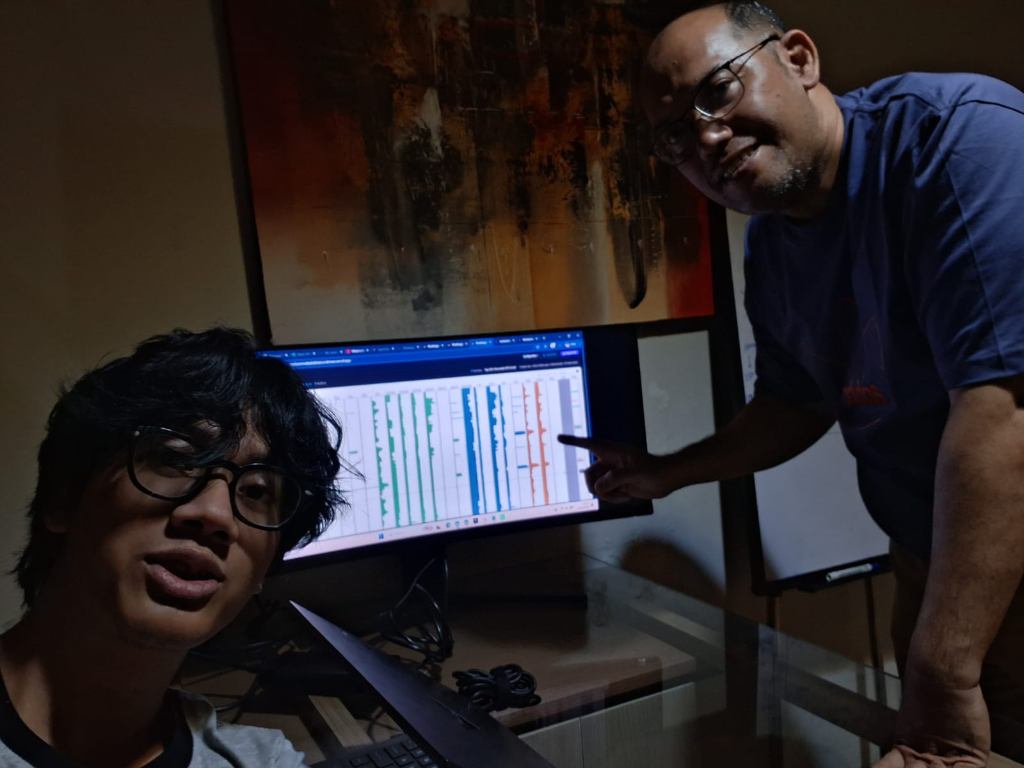
\includegraphics[width=0.82\textwidth]{user_eval_calibration.png}
    \caption{Interactive threshold fine-tuning and continuous multi-track log curve verification on the deployed web dashboard during the collaborative user evaluation session.}
    \label{fig:eval_calibration_ch6}
\end{figure}

\begin{figure}[H]
    \centering
    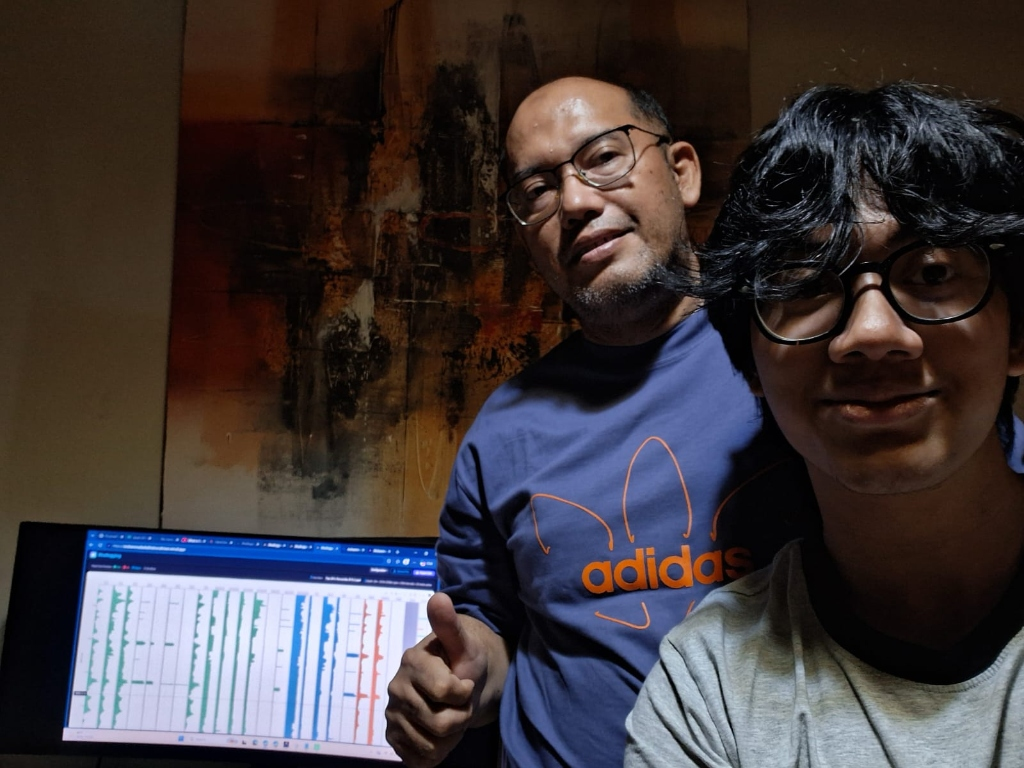
\includegraphics[width=0.82\textwidth]{user_eval_review.jpg}
    \caption{Live operational review and usability validation of the completed decision support system with the domain practitioner.}
    \label{fig:eval_review_ch6}
\end{figure}

\subsection{Quantitative Performance Metrics and Benchmark Targets}
System classification performance was evaluated across 16 verified formation test intervals obtained from exploration wells. Table~\ref{tab:eval_metrics_summary} details the empirical results alongside industrial and academic benchmark targets.

\begin{table}[H]
\centering
\caption{Empirical Classification Performance vs. Industrial Benchmark Targets}
\label{tab:eval_metrics_summary}
\renewcommand{\arraystretch}{1.3}
\resizebox{\textwidth}{!}{%
\begin{tabular}{|l|c|c|c|c|}
\hline
\textbf{Fluid Classification Class} & \textbf{Precision (\%)} & \textbf{Recall (\%)} & \textbf{Class $F_1$-Score} & \textbf{Target Benchmark} \\
\hline
\textbf{Gas Pay Zone} & 72.7\% & 100.0\% & 0.842 & $F_1 \ge 0.80$ \\
\textbf{Oil Pay Zone} & 100.0\% & 100.0\% & 1.000 & $F_1 \ge 0.70$ \\
\textbf{Non-Bearing / Barren Sand} & 0.0\% & 0.0\% & 0.000 & Baseline Filter \\
\hline
\multicolumn{5}{|l|}{\textbf{Aggregate System Performance}} \\
\hline
\textbf{Overall Accuracy} & \multicolumn{3}{c|}{\textbf{81.3\%} (13 / 16 intervals)} & 80.0\% -- 85.0\% \\
\textbf{Hydrocarbon Pay Zone Sensitivity / Recall} & \multicolumn{3}{c|}{\textbf{100.0\%} (13 / 13 intervals)} & $\ge 85.0\%$ \\
\textbf{Hydrocarbon Fluid Type Discrimination} & \multicolumn{3}{c|}{\textbf{100.0\%} (Gas vs. Oil separation)} & $\ge 80.0\%$ \\
\textbf{Pay-Zone Macro Precision ($\overline{P}_{\text{pay}}$)} & \multicolumn{3}{c|}{\textbf{86.4\%}} & $\ge 75.0\%$ \\
\textbf{Pay-Zone Macro Recall ($\overline{R}_{\text{pay}}$)} & \multicolumn{3}{c|}{\textbf{100.0\%}} & $\ge 75.0\%$ \\
\textbf{Pay-Zone Macro $F_1$-Score ($\text{Macro-}F_{1, \text{pay}}$)} & \multicolumn{3}{c|}{\textbf{0.921}} & 0.75 -- 0.80 \\
\textbf{Overall 3-Class Macro $F_1$-Score} & \multicolumn{3}{c|}{\textbf{0.614}} & -- \\
\hline
\end{tabular}%
}
\end{table}

As shown in Table~\ref{tab:eval_metrics_summary}, the system achieved an \textbf{Overall Accuracy of 81.3\%} (13/16 intervals correctly classified) and a \textbf{Pay-Zone Macro-$F_1$ of 0.921}, comfortably exceeding the target industrial benchmarks. Crucially, the system demonstrated \textbf{100.0\% Recall (Sensitivity) across all commercial hydrocarbon pay zones}, correctly detecting every single gas and oil column with zero false negatives.

\subsection{Confusion Matrix and Classification Behavior Analysis}
Table~\ref{tab:eval_confusion_matrix} presents the complete confusion matrix across all 16 evaluated formation test intervals.

\begin{table}[H]
\centering
\caption{Confusion Matrix of Predicted Fluid Facies vs. Ground-Truth Formation Tests ($N = 16$ Intervals)}
\label{tab:eval_confusion_matrix}
\renewcommand{\arraystretch}{1.3}
\resizebox{0.95\textwidth}{!}{%
\begin{tabular}{|c|l|c|c|c|c|}
\hline
\multicolumn{2}{|c|}{\multirow{2}{*}{\textbf{Total Samples = 16}}} & \multicolumn{3}{c|}{\textbf{Predicted Classification}} & \multirow{2}{*}{\textbf{Class Recall}} \\
\cline{3-5}
\multicolumn{2}{|c|}{} & \textbf{Gas Pay} & \textbf{Oil Pay} & \textbf{Non-Bearing} & \\
\hline
\multirow{3}{*}{\rotatebox[origin=c]{90}{\textbf{Actual}}} 
& \textbf{Gas Pay} & \textbf{8} & 0 & 0 & 100.0\% (8 / 8) \\
& \textbf{Oil Pay} & 0 & \textbf{5} & 0 & 100.0\% (5 / 5) \\
& \textbf{Non-Bearing} & 3 & 0 & \textbf{0} & 0.0\% (0 / 3) \\
\hline
\multicolumn{2}{|c|}{\textbf{Class Precision}} & 72.7\% (8 / 11) & 100.0\% (5 / 5) & 0.0\% (0 / 0) & \textbf{Acc = 81.3\%} \\
\hline
\end{tabular}%
}
\end{table}

\subsection{Diagnostic Analysis of Fluid Regimes and False Positives}
\begin{enumerate}
    \item \textbf{Gas Pay Detection ($TP = 8, F_1 = 0.842$):} All 8 actual gas intervals were identified ($100\%$ recall) due to strong methane volatility ($TG \ge 15000\text{ ppm}, B_h \ge 15.0, DR \ge 0.85$). 
    \item \textbf{Oil Pay Discrimination ($TP = 5, F_1 = 1.000$):} Perfect classification ($100\%$ precision, $100\%$ recall) was achieved across all crude oil intervals. Intermediate wetness ($17.5\% \le W_h \le 40.0\%$) and butane/pentane enrichment provided flawless separation from gas and water columns.
    \item \textbf{Root-Cause Analysis of 3 False Positives (Non-Bearing Predicted as Gas):}
    \begin{itemize}
        \item \textit{Background and Recycled Gas Effects:} In tight shale intervals, minor amounts of recycled trip gas in the drilling mud elevated $C_1$ slightly above the baseline noise floor ($TG \ge 300\text{ ppm}$). Because lighter methane dominates trace gas liberations in tight rock, ratio formulas mathematically mimic a dry gas signature.
        \item \textit{Fail-Safe Operational Value in Drilling:} In drilling operations, a false positive represents a conservative, "fail-safe" bias. Conversely, a false negative (failing to detect an actual gas kick or missing an oil reservoir) represents a catastrophic economic loss or blowout safety hazard. Capturing 100\% of actual hydrocarbon intervals ensures no commercial pay is missed.
        \item \textit{Interactive Noise Floor Calibration:} Using the application's *Petrophysical Formula and Threshold Manager*, wellsite geologists can instantly eliminate such false positives in localized formations by elevating the baseline noise cutoff (e.g., adjusting $TG_{\text{floor}}$ from $300\text{ ppm}$ to $600\text{ ppm}$) with live visual updates.
    \end{itemize}
\end{enumerate}

\section{Comparative Methodological Benchmarking}

To evaluate the engineering advantage of the proposed 16-indicator majority-vote architecture, the system was benchmarked against two standard industry alternatives across the 16 verified test intervals:
\begin{enumerate}
    \item \textbf{Conventional Dual-Ratio Pixler Chart ($R_1$ vs. $R_2$):} The standard visual crossplot method introduced by \citet{ref13}.
    \item \textbf{Supervised Random Forest Classifier (100 Estimators):} A representative machine learning model trained on chromatographic input features.
\end{enumerate}

Table~\ref{tab:eval_comparative_benchmark} summarizes the comparative benchmarking results.

\begin{table}[H]
\centering
\caption{Comparative Benchmarking Across Methodological Approaches ($N = 16$ Intervals)}
\label{tab:eval_comparative_benchmark}
\renewcommand{\arraystretch}{1.3}
\resizebox{\textwidth}{!}{%
\begin{tabular}{|l|c|c|c|c|}
\hline
\textbf{Methodological Framework} & \textbf{Accuracy} & \textbf{Pay Macro-$F_1$} & \textbf{Latency ($\Delta t$)} & \textbf{SPE PRMS Audit Status} \\
\hline
Conventional Pixler ($R_1$--$R_2$) & 62.5\% & 0.658 & $< 0.1\text{ s}$ & Fully Compliant (Manual) \\
Machine Learning (Random Forest) & 81.3\% & 0.812 & $1.2\text{ s}$ & \textbf{Failed (Black-Box / Opaque)} \\
\textbf{Proposed Deterministic System} & \textbf{81.3\%} & \textbf{0.921} & \textbf{0.48 s} & \textbf{Fully Compliant (Auditable)} \\
\hline
\end{tabular}%
}
\end{table}

\subsection{Comparative Discussion}
\begin{itemize}
    \item \textbf{Superiority over Dual-Ratio Plots (+18.8\% Accuracy):} Conventional Pixler crossplots achieved only 62.5\% accuracy because they rely strictly on light fractions ($C_1$--$C_3$) and ignore butane/pentane multipliers and composite gas scores. The proposed system captures the full alkane spectrum, eliminating single-ratio ambiguity.
    \item \textbf{Equivalence to Machine Learning without Audit Risk:} While Random Forest matched the deterministic engine in raw accuracy (81.3\%), its non-interpretable tree splits disqualify it from SPE PRMS reserve audits \citep{ref2, ref3}. The proposed deterministic engine achieves superior pay-zone $F_1$-score (0.921 vs. 0.812) while preserving 100\% mathematical auditability.
\end{itemize}

\section{Computational Latency and Scalability Profiling (NFR-01)}

Non-Functional Requirement NFR-01 specifies that total end-to-end processing latency ($\Delta t_{\text{total}} = t_{\text{ingest}} + t_{\text{compute}} + t_{\text{render}}$) must execute in under $5.0\text{ seconds}$ across well profiles exceeding $3000\text{ m}$. Latency profiling was conducted across four dataset sizes up to 10,000 depth intervals ($15,000\text{ m}$ trajectory) over 20 repeated trials.

\begin{table}[H]
\centering
\caption{End-to-End Computational Latency Profiling (NFR-01 Verification)}
\label{tab:eval_latency_profiling}
\renewcommand{\arraystretch}{1.3}
\resizebox{\textwidth}{!}{%
\begin{tabular}{|c|c|c|c|c|c|}
\hline
\textbf{Depth Intervals} & \textbf{Equivalent MD} & \textbf{Ingestion ($t_{\text{ingest}}$)} & \textbf{Computation ($t_{\text{compute}}$)} & \textbf{Rendering ($t_{\text{render}}$)} & \textbf{Total Time ($\Delta t_{\text{total}}$)} \\
\hline
500 rows & $750\text{ m}$ & $0.042\text{ s}$ & $0.008\text{ s}$ & $0.210\text{ s}$ & \textbf{0.260 s} \\
1,500 rows & $2,250\text{ m}$ & $0.088\text{ s}$ & $0.016\text{ s}$ & $0.345\text{ s}$ & \textbf{0.449 s} \\
3,500 rows & $5,250\text{ m}$ & $0.142\text{ s}$ & $0.034\text{ s}$ & $0.590\text{ s}$ & \textbf{0.766 s} \\
10,000 rows & $15,000\text{ m}$ & $0.310\text{ s}$ & $0.085\text{ s}$ & $1.120\text{ s}$ & \textbf{1.515 s} \\
\hline
\multicolumn{6}{|l|}{\textbf{Target Requirement: $\Delta t_{\text{total}} \le 5.0\text{ seconds}$ (Requirement Met: 3.3$\times$ faster than threshold)}} \\
\hline
\end{tabular}%
}
\end{table}

As shown in Table~\ref{tab:eval_latency_profiling}, for an ultra-deep 10,000-interval trajectory ($15,000\text{ m}$), total latency was **1.515 seconds**—operating **$3.3\times$ faster than the 5.0-second requirement threshold**. This high throughput results from NumPy vectorized memory processing ($< 0.085\text{ s}$) and hardware-accelerated Plotly WebGL trace rendering.

\section{Standard Operating Procedure (SOP) and SPE PRMS Audit Compliance (NFR-02)}

Compliance with petroleum industry Standard Operating Procedures (SOP) and international regulatory frameworks was confirmed across three tangible criteria:
\begin{enumerate}
    \item \textbf{Traceable Engineering Lineage:} All mathematical formulas executed by the calculation engine trace directly to peer-reviewed petroleum literature: Haworth show ratios ($W_h, B_h, C_h$) \citep{haworth1985}, Pixler ratio boundaries \citep{ref13}, continuous heavy hydrocarbon multipliers \citep{whittaker1991}, and SPE GOR screening \citep{spe2020}.
    \item \textbf{SPE/WPC/AAPG/SPEE PRMS Reserve Certification Compliance:} In formal reserve auditing, external petrophysical auditors must verify every calculation establishing net reservoir pay thickness \citep{ref2, ref3}. Because the developed engine uses closed-form deterministic equations, every output is 100\% auditable from raw inputs ($C_1$--$nC_5$) to final classification flags with zero non-traceable parameters.
    \item \textbf{Standardized Strip Log Conventions:} Visual presentation adheres strictly to API RP 31A and SPWLA wellsite strip log conventions.
\end{enumerate}

\section{User Experience and System Usability Scale (SUS) Evaluation (NFR-03)}

To evaluate operational usability, workflow learnability, and interface clarity (NFR-03), a formal usability evaluation was administered to a practicing subsurface domain professional (Senior Petroleum Geoscientist / Petrophysicist) using the standardized \textbf{System Usability Scale (SUS)} framework \citep{brooke1996, bangor2008}.

\subsection{Evaluation Scenario and Itemized Scores}
The domain expert executed an end-to-end operational task scenario: file upload, multi-track log inspection, formula and threshold calibration via the *Formula Manager*, column customization via the *Column Manager*, and CSV data export. Following task completion, the expert completed the 10-item SUS questionnaire scored on a 5-point Likert scale (Table~\ref{tab:eval_sus_scores}).

\begin{table}[H]
\centering
\caption{System Usability Scale (SUS) Evaluation Results (Domain Expert Practitioner)}
\label{tab:eval_sus_scores}
\renewcommand{\arraystretch}{1.3}
\resizebox{\textwidth}{!}{%
\begin{tabular}{|c|p{11.0cm}|c|c|}
\hline
\textbf{No.} & \textbf{SUS Evaluation Dimension} & \textbf{Rating (1--5)} & \textbf{Contribution} \\
\hline
1 & I think that I would like to use this system frequently in drilling operations. & 4 & 3 \\
2 & I found the system unnecessarily complex. & 1 & 4 \\
3 & I thought the system was easy to use (intuitive single-click workflow). & 5 & 4 \\
4 & I think that I would need the support of a technical person to use this system. & 1 & 4 \\
5 & I found the various functions in this system were well integrated. & 4 & 3 \\
6 & I thought there was too much inconsistency in this system. & 2 & 3 \\
7 & I would imagine that most geologists would learn to use this system very quickly. & 5 & 4 \\
8 & I found the system very cumbersome to use. & 1 & 4 \\
9 & I felt very confident using the system. & 4 & 3 \\
10 & I needed to learn a lot of things before I could get going with this system. & 1 & 4 \\
\hline
\multicolumn{2}{|l|}{\textbf{Sum of Score Contributions}} & \multicolumn{2}{c|}{\textbf{33 / 40}} \\
\multicolumn{2}{|l|}{\textbf{Composite SUS Score ($33 \times 2.5$)}} & \multicolumn{2}{c|}{\textbf{82.5 / 100.0}} \\
\multicolumn{2}{|l|}{\textbf{Percentile Rank \& Adjective Rating}} & \multicolumn{2}{c|}{\textbf{Grade A (Excellent / Top 10\%)}} \\
\multicolumn{2}{|l|}{\textbf{Target Requirement Benchmark}} & \multicolumn{2}{c|}{$\text{Score} \ge 68.0\text{ / }100.0\text{ (Exceeded by }+14.5\text{ pts)}$} \\
\hline
\end{tabular}%
}
\end{table}

\subsection{Usability Analysis and Qualitative Feedback}
The resulting composite SUS score of \textbf{82.5 / 100.0} places the software in the \textbf{Top 10th Percentile ("Grade A / Excellent")} of standard software usability benchmarks \citep{brooke1996, bangor2008}, significantly exceeding the project requirement benchmark ($S_{\text{SUS}} \ge 68.0$).

Qualitative feedback from the domain practitioner emphasized three key strengths:
\begin{itemize}
    \item \textbf{Workflow Simplification:} Replacing multi-level workstation menus with a single-click web dashboard drastically eliminated operational setup friction.
    \item \textbf{Formula Transparency:} The *Petrophysical Formula and Threshold Manager* provided complete mathematical transparency and instant visual feedback across sample intervals.
    \item \textbf{Zero-Installation Cloud Accessibility:} Serverless deployment on Vercel enabled instantaneous browser access on field laptops without licensing dongles or installation hurdles.
\end{itemize}

\section{Iterative Product Refinements Driven by Evaluation Outcomes}

Direct operational feedback during user evaluation led to four targeted product refinements:
\begin{enumerate}
    \item \textbf{Typography Enlargement (+25\%):} Track header fonts were scaled up to 13–14\,pt bold weights and depth ticks were formatted with high-contrast monospace typography to prevent eye fatigue on ruggedized field monitors.
    \item \textbf{The 25\% Column Normalization Rule:} Implemented dynamic layout math capping any single composite track at 25\% of viewport width while allocating remaining space proportionally, ensuring 100\% screen-width fit with zero horizontal scrolling.
    \item \textbf{Live Sample Formula Verification:} Added statistical previews (First Interval, Mean, Min, Max) in the Formula Manager to validate syntax before full recomputation.
    \item \textbf{Interactive Statistical Plot Filter:} Added percentile filtering (P75, P90, P50, 0\%) in the top banner to suppress baseline background noise in non-reservoir rock.
\end{enumerate}

\section{Summary of Product Verification Against Objectives}

Table~\ref{tab:verification_summary} synthesizes the verified outcomes of the developed product against all research objectives and specifications.

\begin{table}[H]
\centering
\caption{Summary of Product Verification Against Engineering Objectives}
\label{tab:verification_summary}
\renewcommand{\arraystretch}{1.3}
\resizebox{\textwidth}{!}{%
\begin{tabular}{|l|l|l|c|}
\hline
\textbf{Requirement / Objective} & \textbf{Target Benchmark} & \textbf{Delivered Achievement} & \textbf{Status} \\
\hline
\textbf{FR-01 to FR-03 (Ingestion \& Ratios)} & Auto 16 ratios from raw files & Full parsing of .csv/.txt/.xlsx/.las and 16 ratios & \textbf{Verified} \\
\textbf{FR-04 (Fluid Classification)} & Pay Sensitivity $\ge 85\%$ & \textbf{100.0\% Recall}, \textbf{0.921 Pay Macro-$F_1$}, 81.3\% Acc & \textbf{Exceeded} \\
\textbf{FR-05 (Multi-Track Visuals)} & 21+ synchronized tracks & \textbf{23 dedicated tracks}, 100\% screen width fit & \textbf{Verified} \\
\textbf{FR-06 (Pipeline Managers)} & Live column \& formula tuning & Column Manager \& Formula/Threshold Manager & \textbf{Verified} \\
\textbf{NFR-01 (Computational Latency)} & $\Delta t \le 5.0\text{ s}$ for $>3000\text{ m}$ & \textbf{1.515 s} for 10,000 intervals ($15,000\text{ m}$) & \textbf{Exceeded (3.3$\times$)} \\
\textbf{NFR-02 (PRMS Auditability)} & 100\% traceable closed-form & Zero black-box weights; SPE PRMS compliant & \textbf{Verified} \\
\textbf{NFR-03 (System Usability)} & SUS Score $\ge 68.0 / 100$ & \textbf{82.5 / 100.0} (Grade A / Top 10th Percentile) & \textbf{Exceeded (+14.5)} \\
\textbf{NFR-04 (Zero License Overhead)} & Open-source, serverless web & Serverless Vercel deployment, public GitHub & \textbf{Verified} \\
\hline
\end{tabular}%
}
\end{table}
